\documentclass{article}
\usepackage[utf8]{inputenc}
\usepackage{xcolor}
\usepackage{graphicx}
\usepackage{float}
\usepackage{minted}
\usepackage{circuitikz}
\usepackage{tikz}
\usetikzlibrary{shapes, arrows, calc, positioning, circuits.logic.US, circuits.logic.IEC}
\usepackage{geometry}
\geometry{a4paper, margin=1in}
\usepackage{hyperref}
\usemintedstyle{trac}

\usepackage{fancyhdr}
\pagestyle{fancy}
\fancyhf{}
\renewcommand{\headrulewidth}{0pt}
\fancyfoot[C]{\small 010153101 Digital Circuit and Microprocessor Fundamental \\ Semester 2/2025}
\fancyfoot[R]{\thepage}

\fancypagestyle{plain}{%
  \fancyhf{}%
  \fancyfoot[C]{\small 010153101 Digital Circuit and Microprocessor Fundamental \\ Semester 2/2025}%
  \fancyfoot[R]{\thepage}%
  \renewcommand{\headrulewidth}{0pt}%
}

\title{Laboratory Exercise 7 - Week 1 \\ Counters}
\author{}
\date{}

\begin{document}

\maketitle

The purpose of this exercise is to build and use counters. The designed circuits are to be implemented on an Intel FPGA DE0-CV Board.

\section*{Part I}

Consider the circuit in Figure \ref{fig:counter_struct}. It is a 4-bit synchronous counter which uses four T-type flip-flops. The counter increments its value on each positive edge of the clock if the Enable signal is high. The counter is reset to 0 on the next positive clock edge if the asynchronous Clear input is low. You are to implement an 8-bit counter of this type.

\begin{figure}[H]
    \centering
    \resizebox{0.7\textwidth}{!}{\begin{circuitikz}[american]
    % Settings
    \ctikzset{logic ports=ieee, scale=0.8}
    \ctikzset{flipflops/scale=0.8}

    % Parameters
    \def\ffdist{5.5}
    \def\gatey{1.5}

    % Inputs
    \node (clk_in) at (-2, -3) {Clock};
    \node (clr_in) at (-2, -3.5) {Clear};
    \node (enable) at (-2, 0) {Enable};

    % Flip-Flops
    \foreach \i  in {0,1,2,3} {
        \node[flipflop T, anchor=pin 1,flipflop def={nd=1}] (FF\i) at (\i*\ffdist, 0) {};
        \ifnum\i<3
        \node[and port,anchor=in 2] (AND\i) at (FF\i.pin 6) {};
        \draw (FF\i.down) to[short,-*] (FF\i.down |- clr_in.east);
        \draw (FF\i.pin 3) to[short,-*] (FF\i.pin 3 |- clk_in.east);
        \draw (AND\i.in 1) |- ++(-2.5, 0.5) coordinate (Tin\i);
        \fi
    }

    % Bus Lines
    \draw (clk_in.east) -| (FF3.pin 3);
    \draw (clr_in.east) -| (FF3.down);

    % Logic Connections

    % FF0: T = Enable
    \draw (enable.east) -- (FF0.pin 1);

    \foreach \i [evaluate=\i as \nexti using int(\i+1)] in {0,1,2} {
        \ifnum\i>0
        \draw (Tin\i) |- (FF\i.pin 1);
        \fi

        \ifnum\i<2
        \draw (AND\i.out) to[short,-*] (AND\i.out -| Tin\nexti);
        \fi
    }

    \draw (Tin0) to[short,-*] (Tin0 |- FF0.pin 1);
    \draw (AND2.out) -- ++(0.2,0) |- (FF3.pin 1);

  

    

\end{circuitikz}
}
    \caption{A 4-bit synchronous counter using T-type flip-flops.}
    \label{fig:counter_struct}
\end{figure}

perform the following steps:
\begin{enumerate}
    \item Write a VHDL file that defines an 8-bit counter by using the structure depicted in Figure \ref{fig:counter_struct}. Your code should include a T flip-flop entity that is instantiated 8 times to create the counter.
    \item Compile the circuit. How many logic elements (LEs) are used to implement your circuit?
    \item Simulate your circuit to verify its correctness.
    \item Augment your VHDL file to use the pushbutton KEY0 as the Clock input and switches SW1 and SW0 as Enable and Clear inputs, and 7-segment displays HEX1-0 to display the hexadecimal count as your circuit operates.
    \item Download your circuit into the FPGA chip and test its functionality.
\end{enumerate}

\begin{figure}[H]
    \centering
    \resizebox{0.7\textwidth}{!}{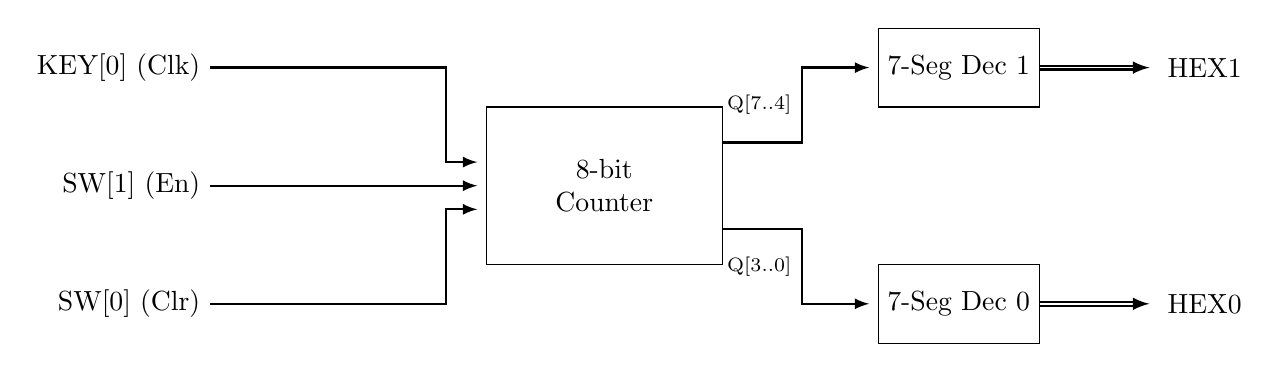
\begin{tikzpicture}[auto, node distance=1.5cm, >=latex]
    % Internal Block: 8-bit Counter (Centered)
    \node [draw, minimum width=3cm, minimum height=2cm, align=center, fill=white] (counter) at (0,0) {8-bit \\ Counter};

    % Inputs - Place relative to Counter
    \node [left=of counter.west, anchor=east, yshift=1.5cm, xshift=-2cm] (key0) {KEY[0] (Clk)};
    \node [left=of counter.west, anchor=east, yshift=0cm, xshift=-2cm] (sw1) {SW[1] (En)};
    \node [left=of counter.west, anchor=east, yshift=-1.5cm, xshift=-2cm] (sw0) {SW[0] (Clr)};

    % Input Connections
    % Route: Input -> (x_turn, input_y) -> (x_turn, target_y) -> Target
    \coordinate (key0_turn) at ($(counter.west) + (-0.5, 0)$);
    \draw [->, thick, shorten >= 3pt] (key0.east) -- (key0.east -| key0_turn) |- ($(counter.west) + (0, 0.3)$);
    \draw [->, thick, shorten >= 3pt] (sw1.east) -- (sw1.east -| key0_turn) -- (counter.west);
    \draw [->, thick, shorten >= 3pt] (sw0.east) -- (sw0.east -| key0_turn) |- ($(counter.west) + (0, -0.3)$);

    % Internal: Decoders
    \node [draw, minimum width=1.5cm, minimum height=1cm, fill=white] (dec0) at (4.5, -1.5) {7-Seg Dec 0};
    \node [draw, minimum width=1.5cm, minimum height=1cm, fill=white] (dec1) at (4.5, 1.5) {7-Seg Dec 1};

    % Counter to Decoders
    \coordinate (counter_turn) at ($(counter.east) + (1, 0)$);
    \draw [->, thick, shorten >= 3pt] (counter.20) -| node[left, font=\scriptsize, near end] {Q[7..4]} (dec1.west -| counter_turn) -- (dec1.west);
    \draw [->, thick, shorten >= 3pt] (counter.340) -| node[left, font=\scriptsize, near end] {Q[3..0]} (dec0.west -| counter_turn) -- (dec0.west);

    % Outputs
    \node [right=of dec1.east] (hex1) {HEX1};
    \node [right=of dec0.east] (hex0) {HEX0};

    % Component to Output Connections
    \draw [->, thick, double, shorten >= 3pt] (dec1.east) -- (hex1.west);
    \draw [->, thick, double, shorten >= 3pt] (dec0.east) -- (hex0.west);

\end{tikzpicture}
}
    \caption{Top-level block diagram of the 8-bit counter.}
    \label{fig:part1_top_level}
\end{figure}

The code for the T flip-flop entity is shown in Figure \ref{fig:t_ff_code}.
For the top-level entity, refer to the block diagram in Figure \ref{fig:part1_top_level}.

\begin{figure}[H]
    \centering
    \begin{minted}[frame=single, fontsize=\small, linenos]{vhdl}
LIBRARY ieee;
USE ieee.std_logic_1164.all;

ENTITY t_ff IS
    PORT ( T, Clk, Clear : IN STD_LOGIC;
           Q : OUT STD_LOGIC);
END t_ff;

ARCHITECTURE Behavior OF t_ff IS
    SIGNAL Q_int : STD_LOGIC;
BEGIN
    PROCESS ( Clk, Clear )
    BEGIN
        IF Clear = '0' THEN
            Q_int <= '0';
        ELSIF RISING_EDGE(Clk) THEN
            IF T = '1' THEN
                Q_int <= NOT Q_int;
            END IF;
        END IF;
    END PROCESS;
    Q <= Q_int;
END Behavior;
    \end{minted}
    \caption{T flip-flop with asynchronous clear.}
    \label{fig:t_ff_code}
\end{figure}

\section*{Part II}

Another way to specify a counter is by using a register and adding 1 to its value. This can be accomplished using the \texttt{ieee.numeric\_std} library and the \texttt{unsigned} type.

\begin{enumerate}
    \item Write a VHDL file for a 16-bit counter using the following statement: \texttt{Q <= Q + 1;}.
    \item Compile the circuit and determine the number of LEs needed.
    \item Use the RTL Viewer to see the structure of this implementation and comment on the differences with the design from Part I.
    \item Implement the counter on your DE0-CV board, using the displays HEX3-0 to show the counter value.
\end{enumerate}

Figure \ref{fig:numeric_std_types} shows how to convert data between different types using \texttt{numeric\_std} library.

\begin{figure}[H]
    \centering
    \resizebox{0.7\textwidth}{!}{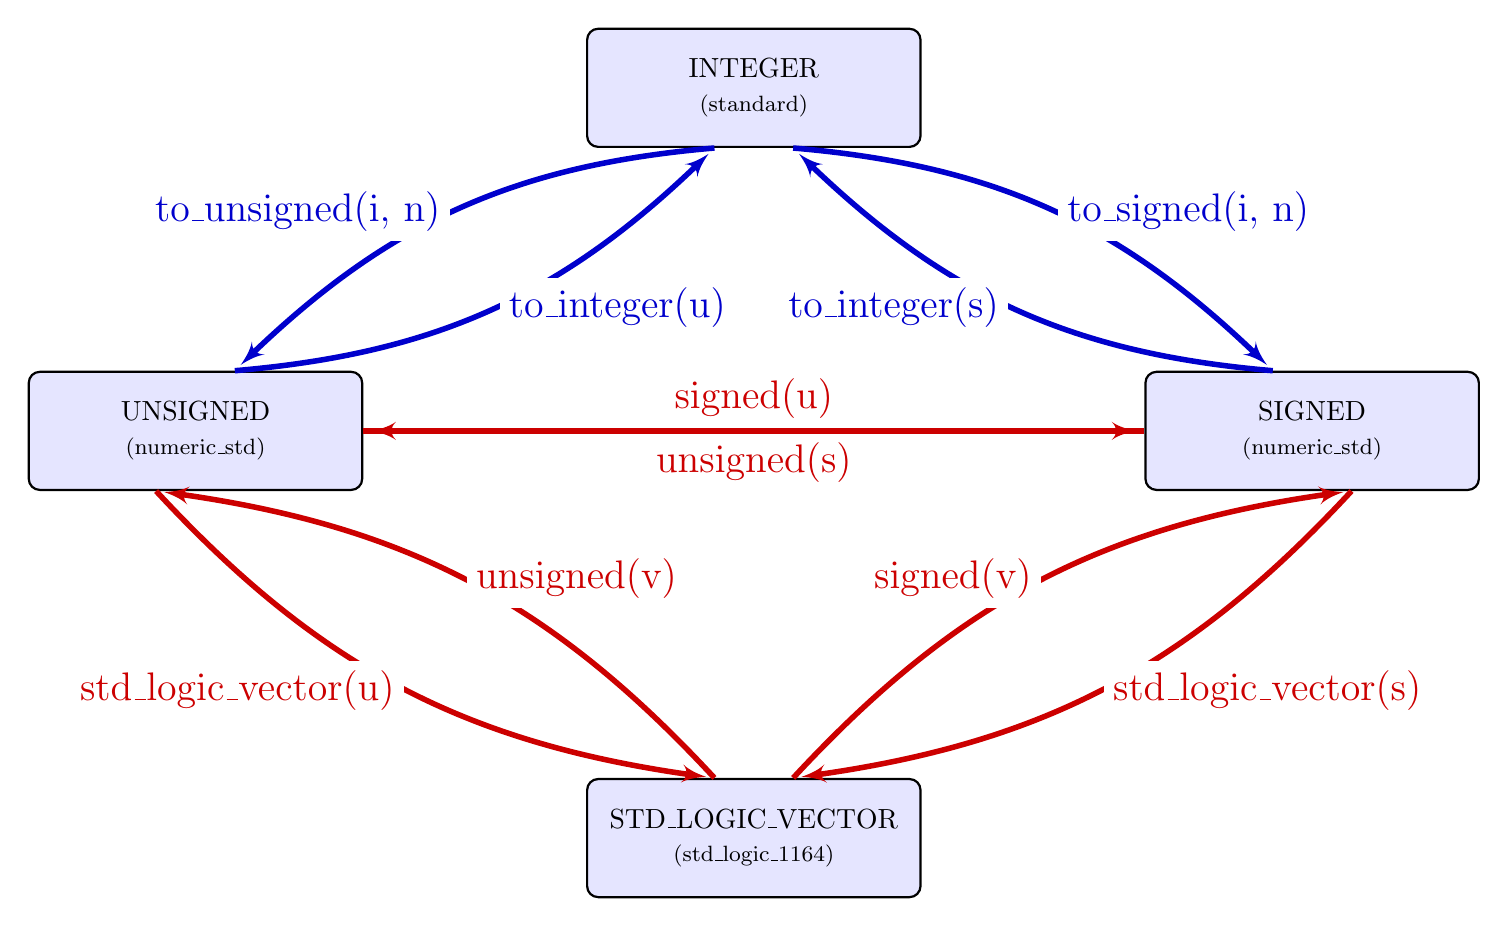
\begin{tikzpicture}[node distance=4cm, auto]
    % Styles
    \tikzstyle{block} = [rectangle, draw, fill=blue!10, text width=4cm, text centered, rounded corners, minimum height=1.5cm, thick]
    \tikzstyle{funcline} = [draw, -latex', line width=2pt, blue!80!black, shorten >=3pt]
    \tikzstyle{castline} = [draw, -latex', line width=2pt, red!80!black, shorten >=3pt]
    \tikzstyle{label} = [midway, fill=white, font=\Large, align=center]

    % Nodes
    \node [block] (int) {INTEGER \\ \footnotesize (standard)};
    \node [block, below left=of int] (uns) {UNSIGNED \\ \footnotesize (numeric\_std)};
    \node [block, below right=of int] (sig) {SIGNED \\ \footnotesize (numeric\_std)};
    \node [block, below=of int, yshift=-4cm] (slv) {STD\_LOGIC\_VECTOR \\ \footnotesize (std\_logic\_1164)};

    % Paths: Integer <-> Unsigned
    \draw [funcline] ([xshift=-0.5cm]int.south) to [bend right=20] node [label, left] {to\_unsigned(i, n)} ([xshift=0.5cm]uns.north);
    \draw [funcline] ([xshift=0.5cm]uns.north) to [bend right=20] node [label, right] {to\_integer(u)} ([xshift=-0.5cm]int.south);

    % Paths: Integer <-> Signed
    \draw [funcline] ([xshift=0.5cm]int.south) to [bend left=20] node [label, right] {to\_signed(i, n)} ([xshift=-0.5cm]sig.north);
    \draw [funcline] ([xshift=-0.5cm]sig.north) to [bend left=20] node [label, left] {to\_integer(s)} ([xshift=0.5cm]int.south);

    % Paths: Unsigned <-> SLV
    \draw [castline] ([xshift=-0.5cm]uns.south) to [bend right=20] node [label, left] {std\_logic\_vector(u)} ([xshift=-0.5cm]slv.north);
    \draw [castline] ([xshift=-0.5cm]slv.north) to [bend right=20] node [label, right] {unsigned(v)} ([xshift=-0.5cm]uns.south);

    % Paths: Signed <-> SLV
    \draw [castline] ([xshift=0.5cm]sig.south) to [bend left=20] node [label, right] {std\_logic\_vector(s)} ([xshift=0.5cm]slv.north);
    \draw [castline] ([xshift=0.5cm]slv.north) to [bend left=20] node [label, left] {signed(v)} ([xshift=0.5cm]sig.south);

    % Paths: Unsigned <-> Signed (Casting)
    \draw [castline] (uns) -- node [label, above] {signed(u)} (sig);
    \draw [castline] (sig) -- node [label, below] {unsigned(s)} (uns);

\end{tikzpicture}
}
    \caption{Data type conversions in \texttt{ieee.numeric\_std}.}
    \label{fig:numeric_std_types}
\end{figure}

\begin{figure}[H]
    \centering
    \begin{minted}[frame=single, fontsize=\small, linenos]{vhdl}
LIBRARY ieee;
USE ieee.std_logic_1164.all;
USE ieee.numeric_std.all;

ENTITY part2 IS
    PORT ( Clk, Reset, Enable : IN STD_LOGIC;
           Q : OUT STD_LOGIC_VECTOR(15 DOWNTO 0));
END part2;

ARCHITECTURE Behavior OF part2 IS
    SIGNAL count_val : UNSIGNED(15 DOWNTO 0);
BEGIN
    PROCESS ( Clk )
    BEGIN
        IF RISING_EDGE(Clk) THEN
            IF Reset = '0' THEN
                count_val <= (OTHERS => '0');
            ELSIF Enable = '1' THEN
                count_val <= count_val + 1;
            END IF;
        END IF;
    END PROCESS;
    Q <= STD_LOGIC_VECTOR(count_val);
END Behavior;
    \end{minted}
    \caption{16-bit counter using \texttt{numeric\_std}.}
    \label{fig:part2_code}
\end{figure}

An implementation example of the counter using \texttt{numeric\_std} is provided in Figure \ref{fig:part2_code}.

\section*{Part III}

Use an LPM from the Library of Parameterized modules to implement a 16-bit counter. Choose the LPM options to be consistent with the above design, i.e. with enable and asynchronous clear.

\begin{enumerate}
    \item Create a VHDL file that instantiates \texttt{lpm\_counter}.
    \item Compare this version with the previous designs in terms of LE usage.
    \item Verify using simulation.
\end{enumerate}

\begin{figure}[H]
    \centering
    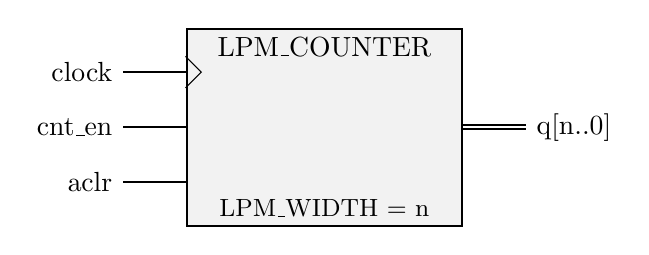
\begin{tikzpicture}
    % LPM Block
    \node [draw, minimum width=3.5cm, minimum height=2.5cm, thick, fill=lightgray!20] (lpm) {};
    
    % Label
    \node [anchor=north] at (lpm.north) {LPM\_COUNTER};
    
    % Inputs
    \draw [thick] (lpm.west) ++(0, 0.7) coordinate (clk_in) -- ++(-0.8, 0) node[anchor=east] {clock};
    \draw (lpm.west) ++(0, 0.5) -- ++(0.2, 0.2) -- ++(-0.2, 0.2); % Clock triangle
    
    \draw [thick] (lpm.west) ++(0, 0) coordinate (cnt_en) -- ++(-0.8, 0) node[anchor=east] {cnt\_en};
    
    \draw [thick] (lpm.west) ++(0, -0.7) coordinate (aclr) -- ++(-0.8, 0) node[anchor=east] {aclr};
    
    % Outputs
    \draw [thick, double] (lpm.east) ++(0, 0) coordinate (q_out) -- ++(0.8, 0) node[anchor=west] {q[n..0]};
    
    % Parameters (Visual representation)
    \node [anchor=south] at (lpm.south) {\small LPM\_WIDTH = n};
\end{tikzpicture}

    \caption{LPM Counter Block.}
    \label{fig:lpm_counter}
\end{figure}
Figure \ref{fig:lpm_counter} shows the LPM counter block representation.



\vspace{1cm}
\noindent \textbf{Updated By:} R. Sutthaweekul \\
\textbf{Release Date:} 2026-01-02

\end{document}
